\documentclass[12pt, a4paper]{amsart} 

\usepackage[T1]{fontenc}    % For fonts
\usepackage{lmodern}    % Font
\usepackage{fullpage}   % For narrower margins to save paper when printing
\usepackage{graphicx}   % For graphics
\usepackage{hyperref}   % For hyperreferencs
\hypersetup{colorlinks=False}
%\usepackage{showframe}  % To show page margins for rough drafts

%\setlength{\hfuzz}{2pt}  % Ignore overlong lines only 2pt over
\pagenumbering{gobble}  % Remove page numbers
\renewcommand{\thefootnote}{\fnsymbol{footnote}}  % Use symbolic footnotes
\graphicspath{{images/}}  % Set path for images
\newcommand{\mi}{\text{i}}  % Math i (= sqrt(-1))
%==============================================================================
\begin{document}
\begin{titlepage}

\noindent
\begin{center}
{\fontsize{2cm}{1em}\selectfont CONTOURS}\\[1.5em]
{\fontsize{0.7cm}{1em}\selectfont\itshape A Mathematical Coloring Book}\\[4em]
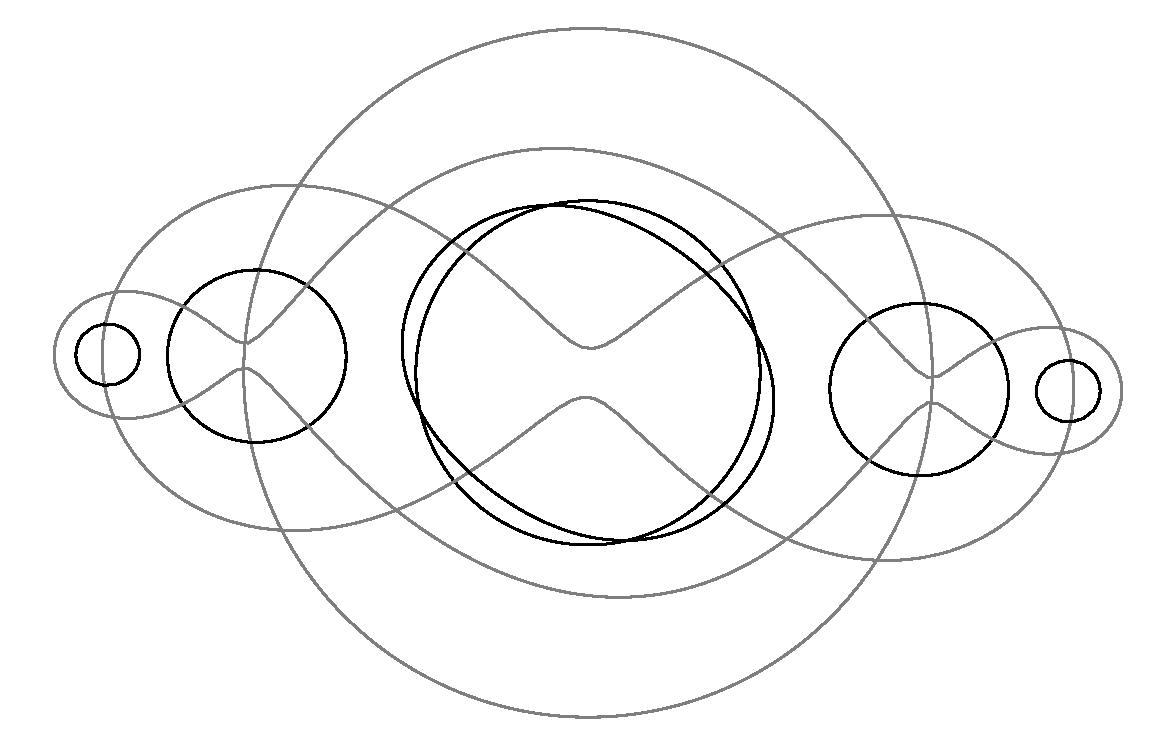
\includegraphics[width=160mm, angle=90]{images/cover.pdf}\\
\vfill
{\fontsize{0.6cm}{1em}\selectfont ALEXANDER RAICHEV}
\end{center}
\end{titlepage}

%-----------------------------------------------------------------------------
\section*{Introduction}

Q: What is this?

A: This is a mathematical coloring book.
It contains black and white pictures generated by mathematical formulas which you color in for fun.

Q: Why did you make it? 

A: I like math and drawing and decided to combine the two.
Also, I was inspired by \cite{Hamp2009}.

Q: Is this book for kids or adults?

A: Both.
The only requirements are sharp pencils and fine motor skills.

Q: What does the title mean? 

A: Every picture in this book is a contour plot.
A contour plot of a three-dimensional object is an overlay of several parallel two-dimensional cross sections of the object, each of which is called a contour line or contour.
You can think of the object as a landscape and the contour plot as a topographical map of that landscape.

Q: How did you make these pictures?

A: For each picture I chose a function from the plane to the plane, computed several of its iterates, collapsed the outputs to the real line, plotted one to three contours of the resulting functions, overlaid them, and then cropped and sometimes rotated and resized the result.
I got this idea from \cite{Hamp2009}.
To make the plots, I used Sage~\cite{Sage}, an open-source mathematics software system.

For example, consider the cover picture.
It is a homage to \cite{Hamp2009}, because it involves a function that appears in that book, namely the complex quadratic function $f(z) = z^2  - 0.99 + 0.1\mi$.
Working with a complex function simplifies things, because then you can  generate a mapping from the plane to the plane by a formula using only one (complex) variable, instead of two (real) variables.

Because the graph of $f$ is four-dimensional, I took the absolute value of $f$, which can be plotted in three dimensions and therefore yields a two-dimensional contour plot; see Figure~\ref{fig:3d}.

\begin{figure}[!ht]
(a) 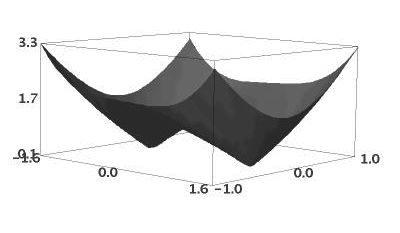
\includegraphics[width=60mm]{images/tutorial_3d.png}\qquad
(b) 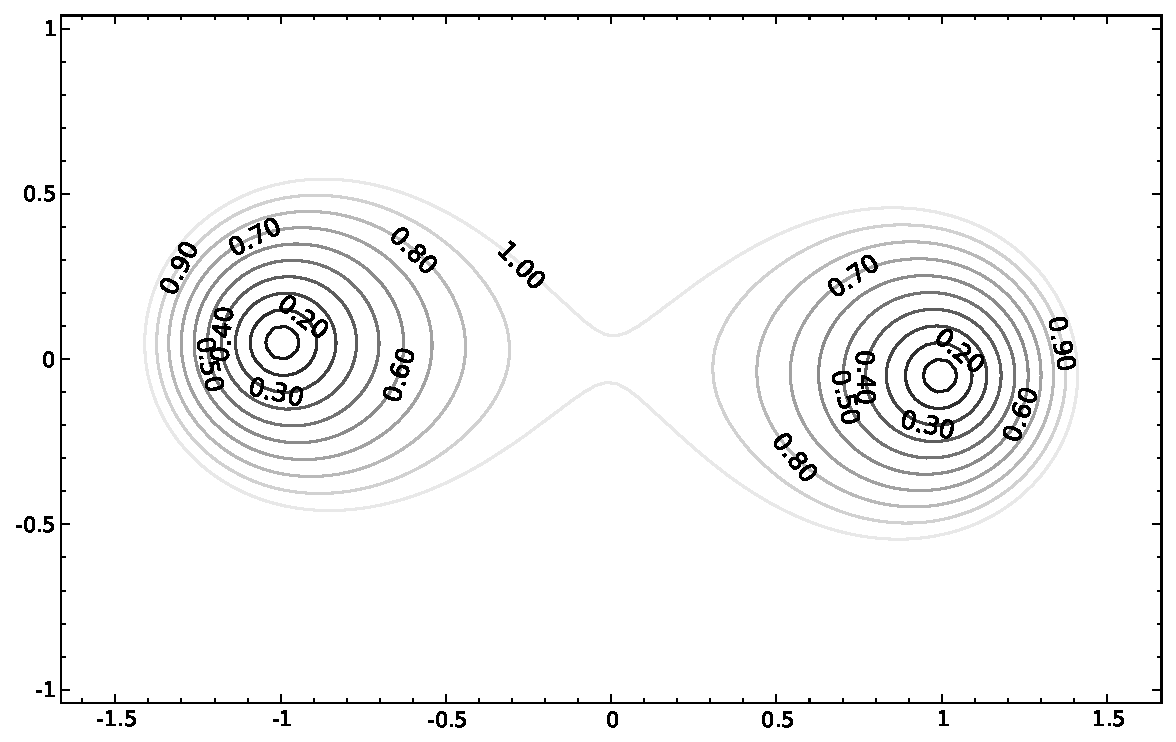
\includegraphics[width=60mm]{images/tutorial_contour.pdf}
\caption{
(a) Plot of $|f(z)|$ for the complex function $f(z) = z^2  - 0.99 + 0.1\mi$
(b) Contour plot of $|f(z)|$ with contour heights labeled
}
\label{fig:3d}
\end{figure}

Now, to my eye that contour plot is too plain for coloring.
It needs variation.
But how to produce that variation in a systematic way?
Overlay iterates of $f$. 
Iterating a function several times, even a simple one, usually produces intricate patterns.
There is even a whole field of mathematics, called dynamical systems, dedicated to studying the behavior of iterated functions.

For this example, I used the zeroth, first, and second iterates of $f$, chose two contours for each iterate, because more than that crowds the picture, overlaid the plots, and cropped the results; see Figure~\ref{fig:iterates}.
Finally, I rotated the picture by 90 degrees.

\begin{figure}[!htb]
(a) 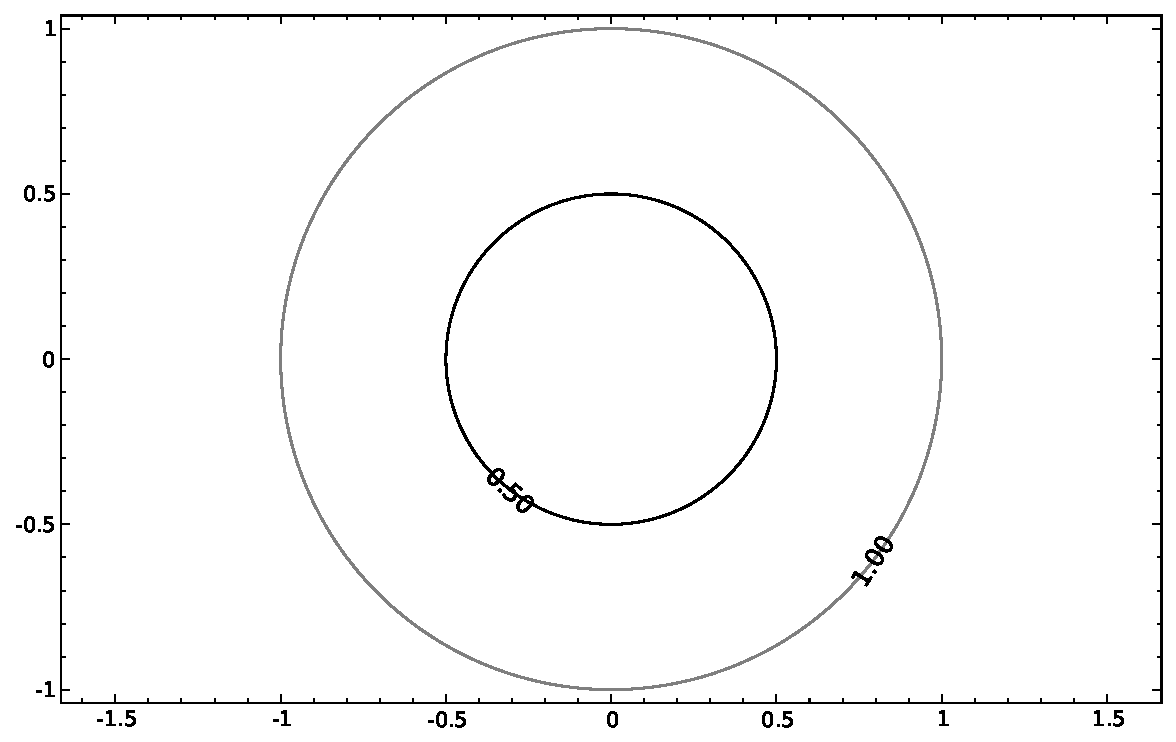
\includegraphics[width=60mm]{images/tutorial_c0.pdf}\qquad
(b) 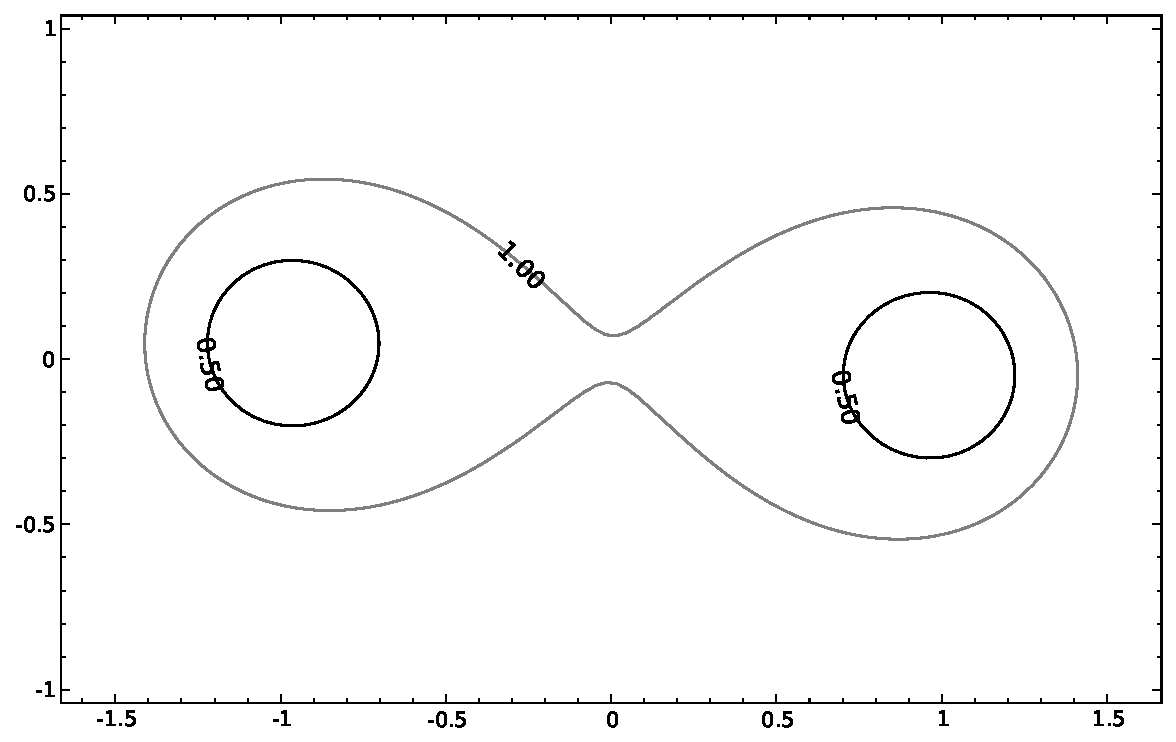
\includegraphics[width=60mm]{images/tutorial_c1.pdf}\\
(c) 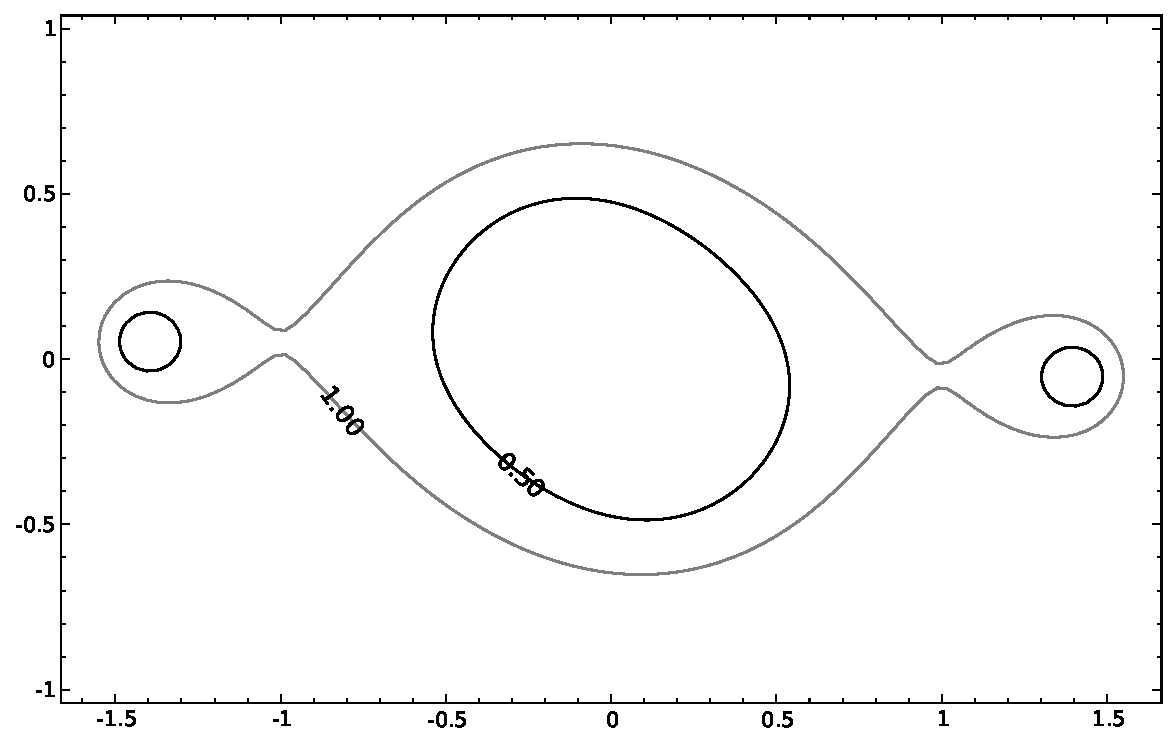
\includegraphics[width=60mm]{images/tutorial_c2.pdf}\qquad
(d) 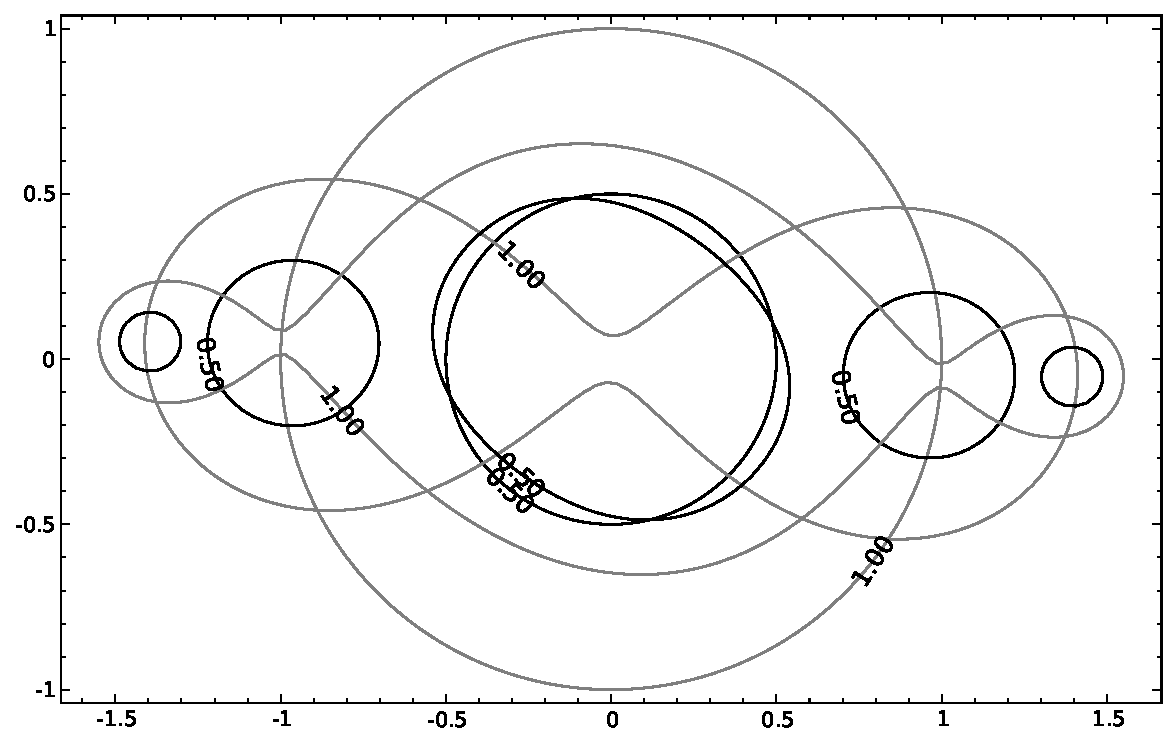
\includegraphics[width=60mm]{images/tutorial_c012.pdf}
\caption{
Labeled contour plots with contours at heights 0.5 and 1.
(a) $|f^{\circ 0}(z)|$ 
(b) $|f^{\circ 1}(z)|$
(c) $|f^{\circ 2}(z)|$
(d) The overlay of (a), (b), and (c)
}
\label{fig:iterates}
\end{figure}

Q: How did you choose the underlying functions?

A: Lots of trial and error and squinting at the screen.
I began with linear and quadratic functions and then sprinkled in more complicated functions for spice, such as the sine function.
I also experimented with several chaotic functions, such as the \href{https://en.wikipedia.org/wiki/Gingerbreadman_map}{Gingerbreadman map}.

There are infinitely many functions to choose from, and the ones in this book are simply the first 11 that I bumped into and found beautiful.

Q: Can I make pictures like these too?

A: You bet!
One quick way to start is to grab the Sage worksheet I used to produce the images in this book from \url{https://github.com/araichev/contours/contours.sws} and play with it via Sage online at \url{http://www.sagenb.org}.
%-----------------------------------------------------------------------------
\section*{Further Reading}

\begin{itemize}
    \item \url{https://en.wikipedia.org/wiki/Contour_plot}
    \item \url{https://en.wikipedia.org/wiki/Complex_function} 
    \item \url{https://en.wikipedia.org/wiki/Dynamical_system}
\end{itemize}
%-----------------------------------------------------------------------------
\section*{Acknowledgements}

Thanks to Poppy Constantine and Sasha Rubin for their constructive feedback.

%-----------------------------------------------------------------------------
\section*{Copyright}

This work was produced 2013-04-03 by Alexander Raichev and is licensed under a \href{http://creativecommons.org/licenses/by-nc-sa/4.0/}{Creative Commons Attribution-NonCommercial-ShareAlike 4.0 International License}.
%
\includegraphics[width=20mm]{cc_by_sa.png}

%-----------------------------------------------------------------------------
\bibliographystyle{amsalpha}
\bibliography{contours}
\vfill
%-----------------------------------------------------------------------------
\pagebreak
\begin{figure}[!ht]
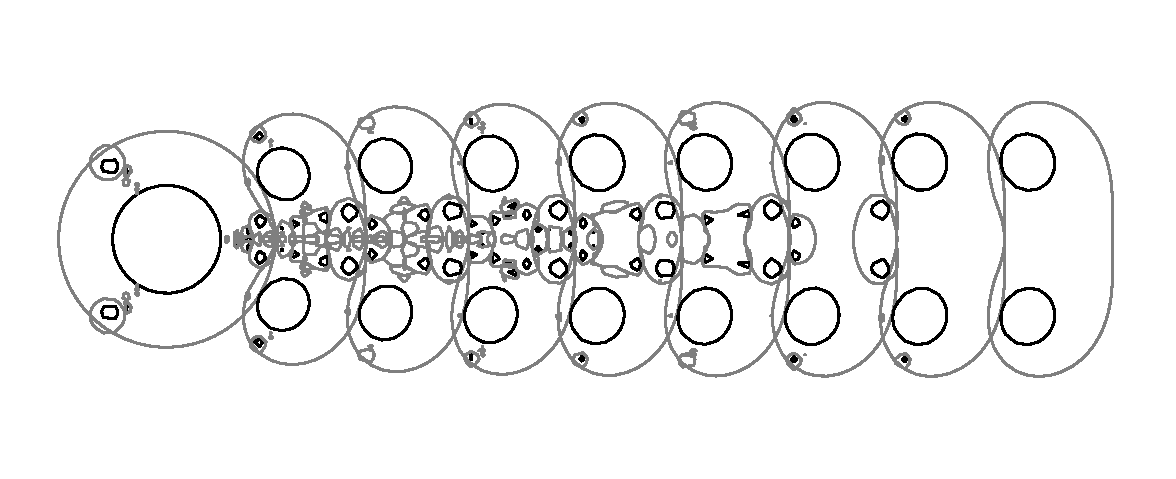
\includegraphics[width=230mm, angle=-90]{images/caterpillar.pdf}
\caption{
Contour plot of $|f^{\circ j}(z)|$ for $j = 0, 1, \ldots, 8$ and the complex function $f(z) = z - 1 + 1/z^3$.
Contour heights 0.5 and 1.
}
\end{figure}
%-----------------------------------------------------------------------------
\pagebreak
\begin{figure}[!ht]
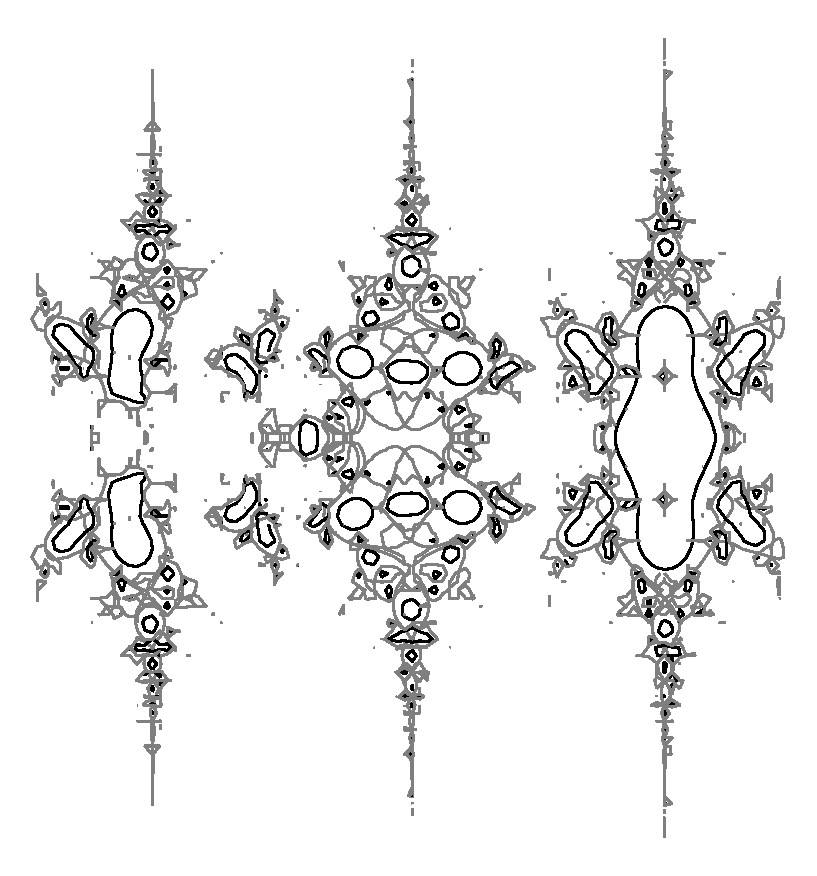
\includegraphics[width=160mm, height=210mm, angle=180]{images/indian_caterpillar.pdf}
\caption{
Contour plot of $|f^{\circ j}(z)|$ for $j = 2, 3, 4$ and the complex function $f(z) = \sin(z - 1 + 1/z^3)$.
Contour heights 0.5 and 1.
}
\end{figure}
%-----------------------------------------------------------------------------
\pagebreak
\begin{figure}[!ht]
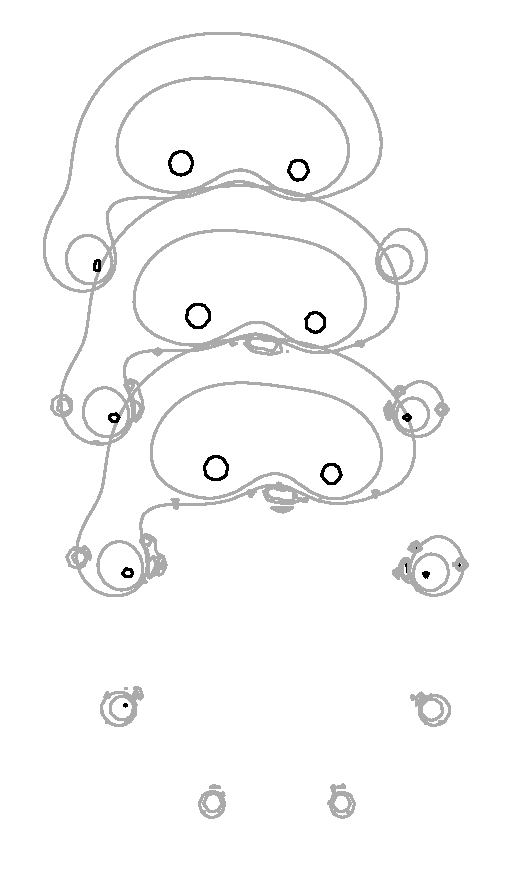
\includegraphics[height=230mm]{images/three_monkeys.pdf}
\caption{
Contour plot of $|f^{\circ j}(z)|$ for $j = 1, 2, 3$ and the complex function $f(z) = z + 1 -0.9\mi + 1/z^7$.
Contour heights 0.2, 0.75, and 1.
}
\end{figure}
%-----------------------------------------------------------------------------
\pagebreak
\begin{figure}[!ht]
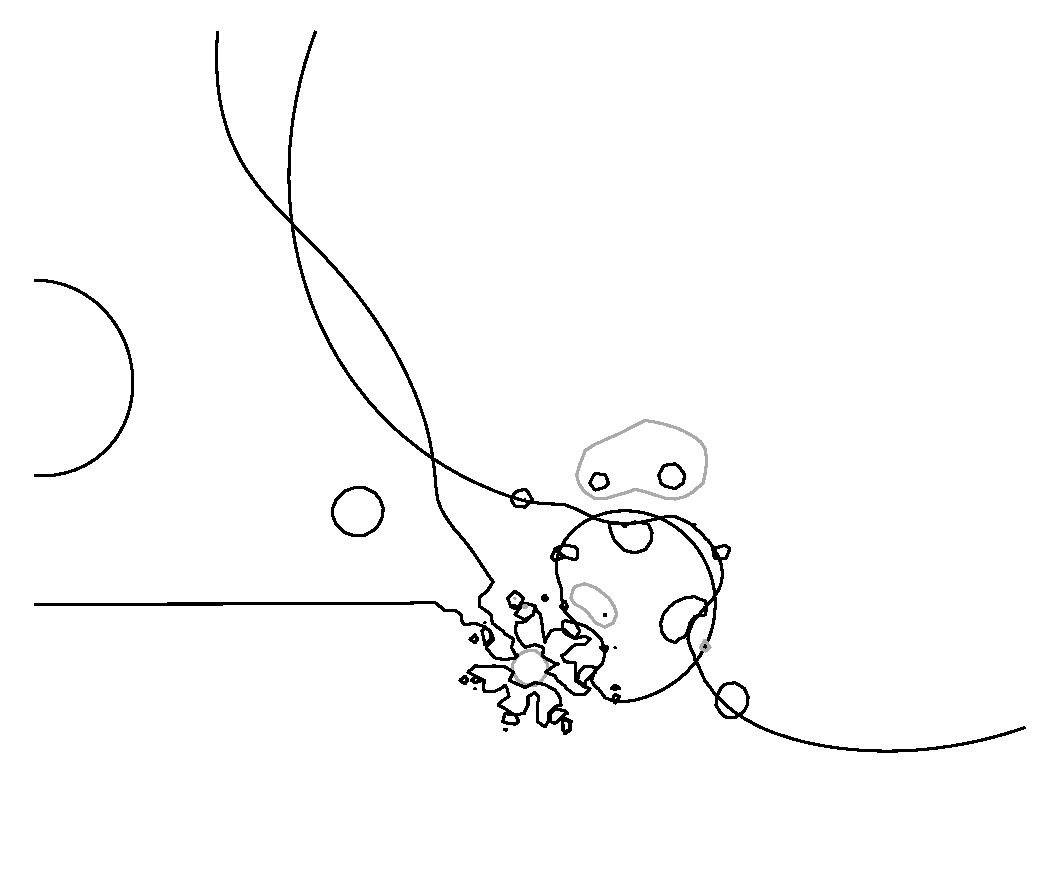
\includegraphics[width=160mm, height=170mm]{images/three_monkeys_eaten.pdf}
\caption{
Contour plot of $|f^{\circ j}(z)|$ for $j = 1, 2, 3$ and the complex function $f(z) = \log(z + 1 -0.9\mi + 1/z^7)$.
Contour heights 0.1, 1, and 10.
}
\end{figure}
%-----------------------------------------------------------------------------
\pagebreak
\begin{figure}[!ht] 
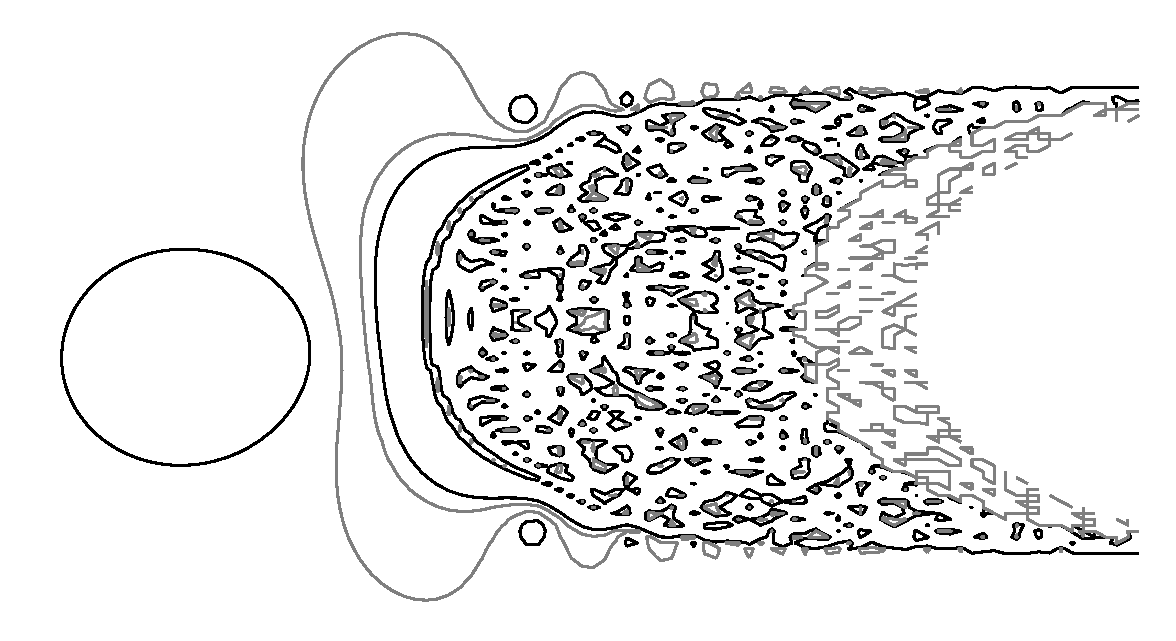
\includegraphics[width=230mm, angle=-90]{images/mr_fancy_pants.pdf}
\caption{
Contour plot of $\sin(|f^{\circ 2}(z)|)$ for the complex function $f(z) = \exp(z) - 0.99 + 0.1\mi$.
Contour heights 0.5 and 0.9.
}
\end{figure}
%-----------------------------------------------------------------------------
\pagebreak
\begin{figure}[!ht]
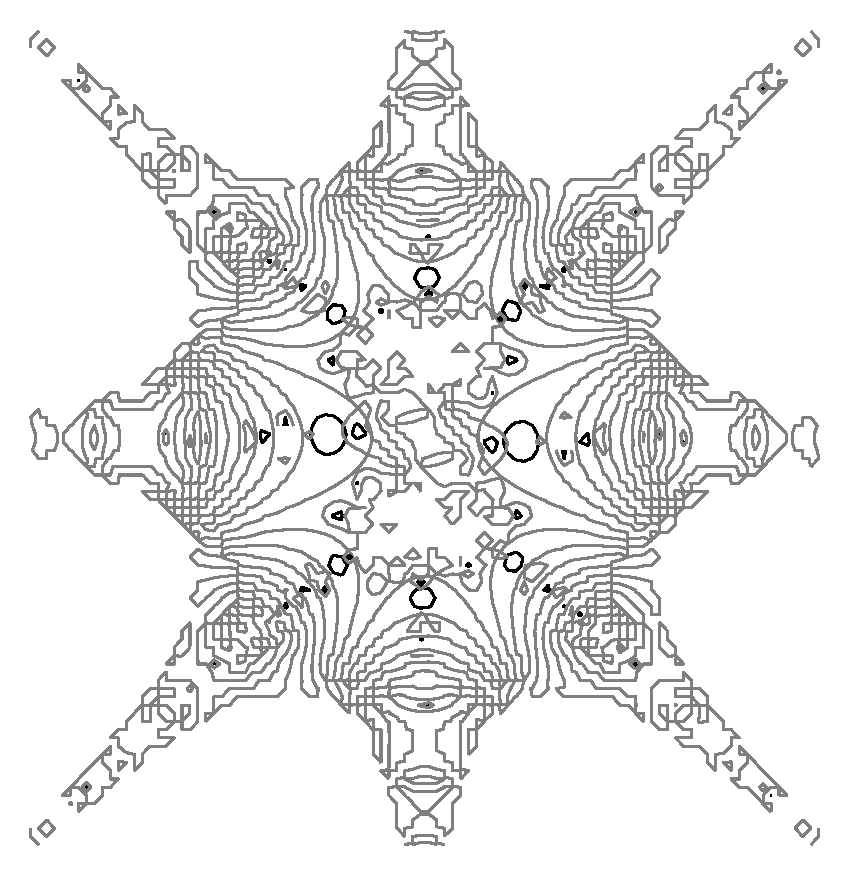
\includegraphics[width=160mm]{images/mite.pdf}\\[10mm]
\caption{
Contour plot of $|f^{\circ j}(z)|$ for $j = 1, 2$ and the complex function $f(z) = \tan(z^2  + z^2 - 0.99 + 0.1\mi)$.
Contour heights 0.5 and 1.
}
\end{figure}
%-----------------------------------------------------------------------------
\pagebreak
\begin{figure}[!ht] 
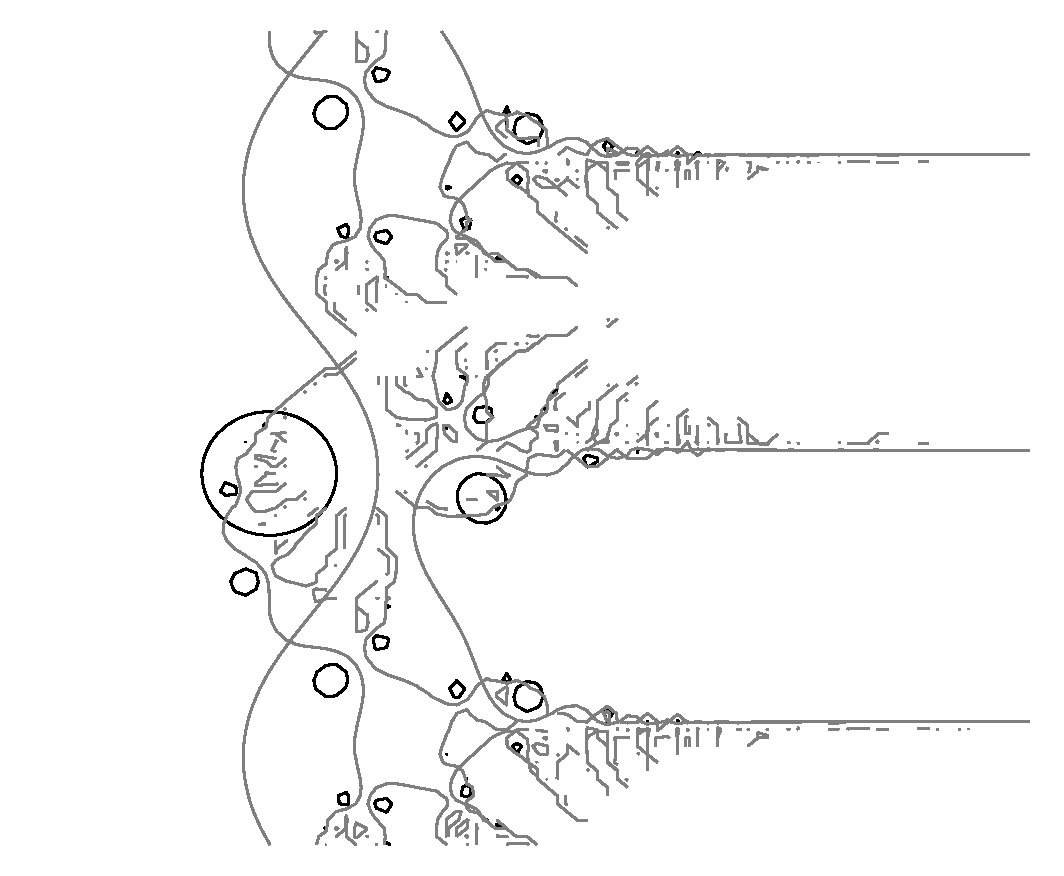
\includegraphics[height=160mm, angle=-90]{images/landscape.pdf}\\[10mm]
\caption{
Contour plot of $|f^{\circ j}(z)|$ for $j=1, 2, \ldots, 7$ and the complex function $f(z) = \exp(z) + 0.1 + 0.3\mi$.
Contour heights 0.2 and 0.5.
}
\end{figure}
%-----------------------------------------------------------------------------
\pagebreak
\begin{figure}[!ht] 
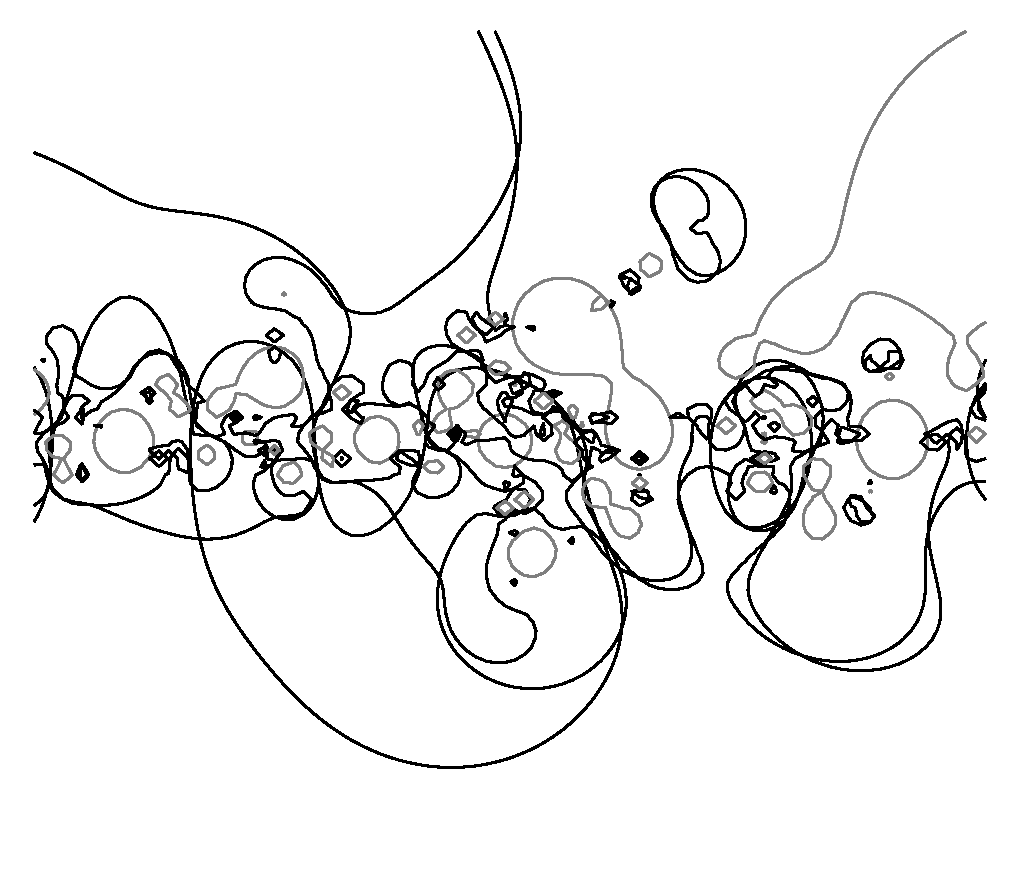
\includegraphics[height=160mm, angle=90]{images/embryos.pdf}\\[10mm]
\caption{
Contour plot of $|f^{\circ j}(z)|$ for $j=1, 2, 3, 4$ and the complex function $f(z) = \cot(z)(1/z - 0.3 + 0.7\mi)$.
Contour heights 1 and 10.
}
\end{figure}
%-----------------------------------------------------------------------------
\pagebreak
\begin{figure}[!ht] 
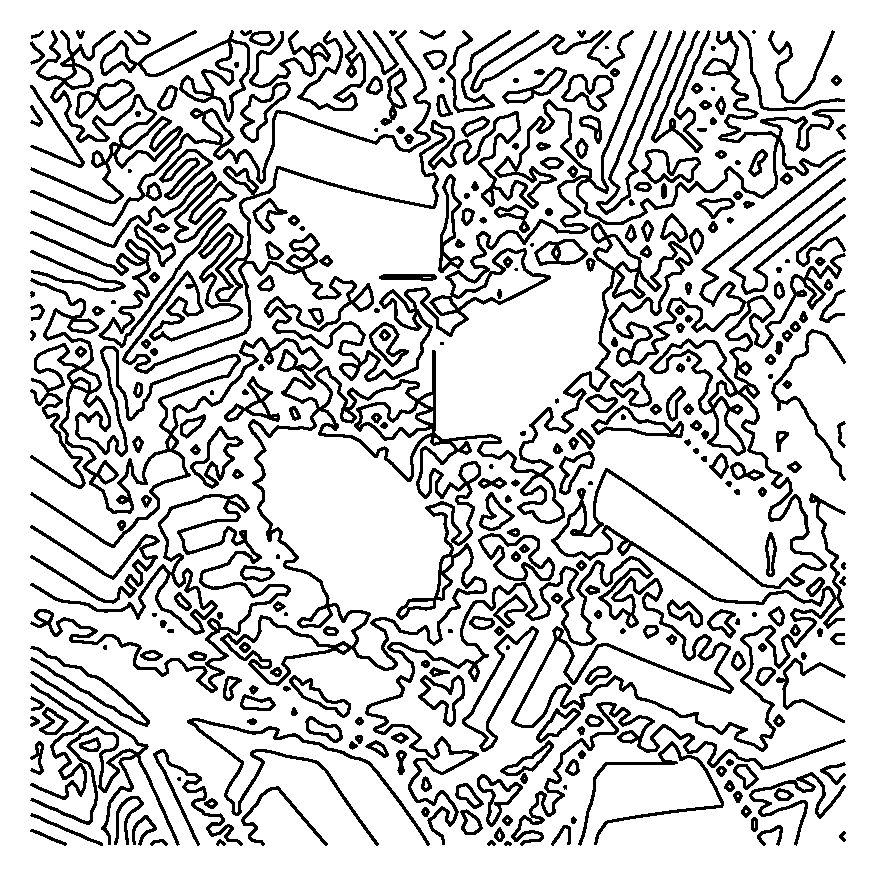
\includegraphics[width=160mm, height=210mm]{images/gingerbreadman.pdf}
\caption{
Contour plot of $\sin(x_{65} y_{65})$ for $(x_{65}, y_{65}) = f^{\circ 65}(x, y)$ and the Gingerbreadman map $f(x, y) = (1 - y + |x|, x)$.
Contour height 0.
}
\end{figure}
%-----------------------------------------------------------------------------
\pagebreak
\begin{figure}[!ht] 
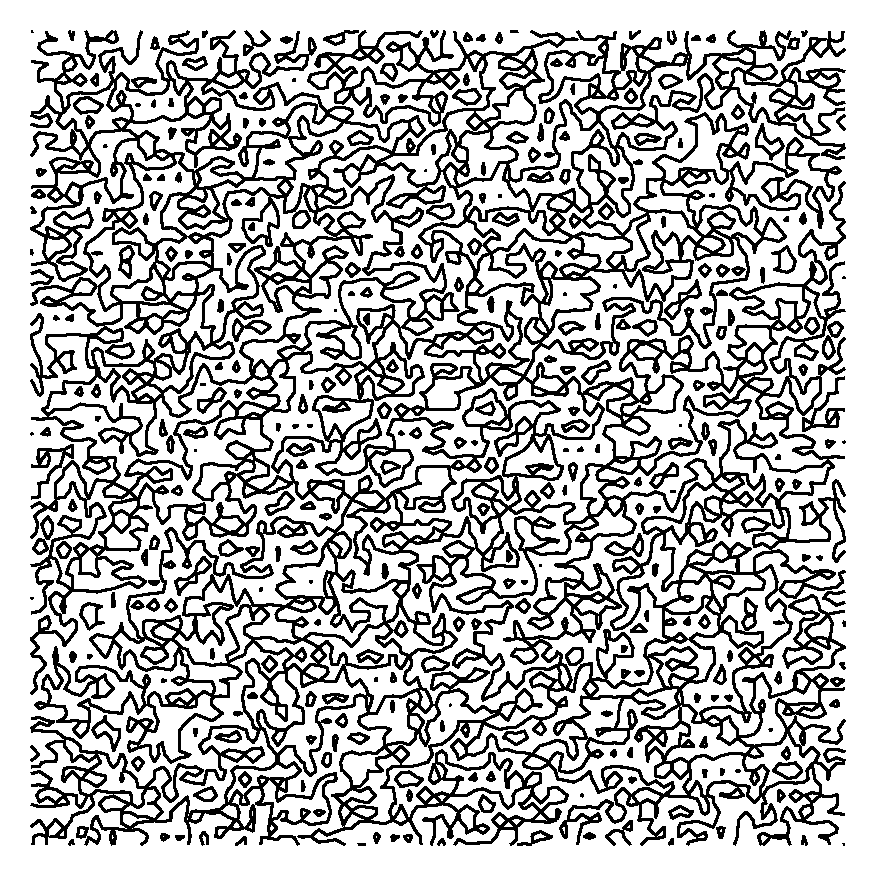
\includegraphics[width=160mm, height=210mm]{images/arnolds_cat.pdf}
\caption{
Contour plot of $\tan(x_8 + y_8)$ for $(x_8, y_8) = f^{\circ 8}(x, y)$ and  $f(x, y) = (2x + (y \mod 3), x + (y \mod 3))$.
Contour height 0.
}
\end{figure}
\end{document}
